%
% The first command in your LaTeX source must be the \documentclass command.
\documentclass[sigconf,anonymous,review,screen]{acmart}
\usepackage{booktabs}
\usepackage{verbatim}
\usepackage{graphicx}
\usepackage{ragged2e}

 %activate todo's
\newcommand{\ld}[1]{ \textcolor{purple}{Laura: #1}}
\newcommand{\todo}[1]{}%\textcolor{red}{TODO: #1}\PackageWarning{TODO:}{#1!}}
% deactivate todos
%\newcommand{\todo}[1]{ \PackageWarning{TODO:}{#1!}}

%
% defining the \BibTeX command - from Oren Patashnik's original BibTeX documentation.
\def\BibTeX{{\rm B\kern-.05em{\sc i\kern-.025em b}\kern-.08emT\kern-.1667em\lower.7ex\hbox{E}\kern-.125emX}}
    
% Rights management information. 
% This information is sent to you when you complete the rights form.
% These commands have SAMPLE values in them; it is your responsibility as an author to replace the commands and values with those provided to you when you complete the rights form.
%
% These commands are for a PROCEEDINGS abstract or paper.
\copyrightyear{2018}
\acmYear{2018}
\setcopyright{acmlicensed}
\acmConference[Woodstock '18]{Woodstock '18: ACM Symposium on Neural Gaze Detection}{June 03--05, 2018}{Woodstock, NY}
\acmBooktitle{Woodstock '18: ACM Symposium on Neural Gaze Detection, June 03--05, 2018, Woodstock, NY}
\acmPrice{15.00}
\acmDOI{10.1145/1122445.1122456}
\acmISBN{978-1-4503-9999-9/18/06}

%
% These commands are for a JOURNAL article.
%\setcopyright{acmcopyright}
%\acmJournal{TOG}
%\acmYear{2018}\acmVolume{37}\acmNumber{4}\acmArticle{111}\acmMonth{8}
%\acmDOI{10.1145/1122445.1122456}

%
% Submission ID. 
% Use this when submitting an article to a sponsored event. You'll receive a unique submission ID from the organizers
% of the event, and this ID should be used as the parameter to this command.
%\acmSubmissionID{123-A56-BU3}

%
% The majority of ACM publications use numbered citations and references. If you are preparing content for an event
% sponsored by ACM SIGGRAPH, you must use the "author year" style of citations and references. Uncommenting
% the next command will enable that style.
%\citestyle{acmauthoryear}

%
% end of the preamble, start of the body of the document source.
\begin{document}

%
% The "title" command has an optional parameter, allowing the author to define a "short title" to be used in page headers.
\title[Entity Aspect Linking]{Entity Aspect Linking: Enriching Entity Links with Fine-Grained Knowledge using Entity Salience and Relatedness}

%
% The "author" command and its associated commands are used to define the authors and their affiliations.
% Of note is the shared affiliation of the first two authors, and the "authornote" and "authornotemark" commands
% used to denote shared contribution to the research.
%\author{Shubham Chatterjee}
%\email{sc1242@cs.unh.edu}
%\orcid{1234-5678-9012}
%\affiliation{
% \institution{University of New Hampshire}
%  \city{Durham}
% \state{New Hampshire}
%}
%\author{Jordan Ramsdell}
%\email{jsc57@cs.unh.edu}
%\orcid{1234-5678-9012}
%\affiliation{
% \institution{University of New Hampshire}
%  \city{Durham}
% \state{New Hampshire}
%}
%\author{Laura Dietz}
%\email{dietz@cs.unh.edu}
%\affiliation{
% \institution{University of New Hampshire}
%  \city{Durham}
% \state{New Hampshire}
%}

%
% By default, the full list of authors will be used in the page headers. Often, this list is too long, and will overlap
% other information printed in the page headers. This command allows the author to define a more concise list
% of authors' names for this purpose.
%\renewcommand{\shortauthors}{Chatterjee et al.}

%
% The abstract is a short summary of the work to be presented in the article.
\begin{abstract}
Entity linking tools had a significant impact on information retrieval. However, entity linking focuses only on the resolution and disambiguation of entities in a knowledge graph. In this work, we augment entity links with more fine-grained information clarifying which aspect of an entity is being referred to in this context. While many definitions of aspects can be leveraged in our formulation, we define Entity Aspect Linking as the task of associating an entity link with one of several known sub-aspects, such as Wikipedia sections.

Several pre-trained entity salience and relatedness detectors are available to predict salient entities in the text or the relatedness of two entities. However, these tools are not trained for our particular task. Salience detection is unaware of the entity's knowledge graph representation and entity relatedness is not considering the context. In this work, we study if and to what extent, such static, off-the-shelf tools can be utilized in the aspect linking task. Our results show that although a static measure of entity salience and relatedness from an off-the-shelf tool works on its own, a supervised combination of these indicators with lexical and semantic features based on the contexts of different sizes around the entity mention provides better results.


%Previous work \cite{nanni2018entity} has shown that a supervised combination of various text and entity features can correctly predict aspects in 70\% of the cases. In this work, we consider the salience of an entity in the aspect (that is, its centrality to the aspect) and its relatedness to other entities and obtain new state-of-the-art results on the task. Moreover, we study the effect of the frequency and relatedness of co-occurring entities with a given entity on the task.
\end{abstract}

\begin{CCSXML}
<ccs2012>
   <concept>
       <concept_id>10002951.10003317.10003338.10003340</concept_id>
       <concept_desc>Information systems~Probabilistic retrieval models</concept_desc>
       <concept_significance>100</concept_significance>
       </concept>
   <concept>
       <concept_id>10002951.10003317.10003338.10003341</concept_id>
       <concept_desc>Information systems~Language models</concept_desc>
       <concept_significance>300</concept_significance>
       </concept>
   <concept>
       <concept_id>10002951.10003317.10003338.10003342</concept_id>
       <concept_desc>Information systems~Similarity measures</concept_desc>
       <concept_significance>500</concept_significance>
       </concept>
 </ccs2012>
\end{CCSXML}

\ccsdesc[100]{Information systems~Probabilistic retrieval models}
\ccsdesc[300]{Information systems~Language models}
\ccsdesc[500]{Information systems~Similarity measures}


% Keywords. The author(s) should pick words that accurately describe the work being presented. Separate the keywords with commas.
\keywords{entities, entity-aspects, wikification, entity salience, entity relatedness, co-occurring entities}

% This command processes the author and affiliation and title information and builds
% the first part of the formatted document.
\maketitle

\section{Introduction}
\label{sec:Introduction}


The larger goal of our work is to support efficient information access on complex topics. 
%
For example, consider a journalist writing an article on the recent Coronavirus Disease 2019 (COVID-19)
pandemic in which she analyzes the different angles of the pandemic on the economy and worker's safety. COVID-19 has been widely discussed in the news, social media, and research commentary in various aspects such as transmission, pathology, experimental treatment, food safety, protests, and stay-at-home-orders. So the journalist has to sift through hundreds of associated texts to identify those that discuss the right context. The journalist finds it challenging to identify different texts that are relevant for her article without being overwhelmed with other aspects of COVID-19. Of course, keyword searches help her, but she would also like to understand the larger connections between her topic and other policies, research findings, and incidents. One relevant text passage for her task is displayed in Figure \ref{fig:introexample}, top. 



\begin{figure}
\justify
\begin{quote}
Several \textbf{meat processing plants} around the \textbf{U.S.} are sitting idle this week because workers have been infected with the \textbf{coronavirus}. \textbf{Tyson Foods}, one of the country's biggest \textbf{meat processors}, says it suspended \textbf{operations} at its \textbf{pork plant} in \textbf{Columbus Junction, Iowa}, after more than two dozen workers got sick with \textbf{COVID-19}. \textbf{National Beef Packing} stopped \textbf{slaughtering} \textbf{cattle} at another \textbf{Iowa} plant, and \textbf{JBS USA} shut down work at a \textbf{beef plant} in \textbf{Pennsylvania}.
\end{quote}

\begin{small}
\begin{itemize}
\item Meat packing industry:  Meatpackers / Today
\item United States: Culture / Food
\item Coronavirus Disease 2019: Cause / Transmission
\item Tyson Foods: Controversies / Coronavirus (COVID-19) pandemic
\item Continuous production: Shut-downs / Safety
\item Columbus Junction, Iowa: History
\item National Beef: Food Safety
\item Cattle: Economy / Cattle meat production
\item Iowa: Economy / Manufacturing
\item Meat Industry: Effects on Livestock Workers
\item Animal Slaughter: National laws / United States
\item JBS USA: Coronavirus Outbreak
\item Pennsylvania: Economy / Agriculture
\end{itemize}
\end{small}


\caption{Entity Aspect Linking Example. Top: An example paragraph about a COVID-19 outbreak in the meat packing industry, where the entity [Coronavirus Disease 2019] is mentioned with its aspect ``transmission''.  Bottom: Entities mentioned in text with their referenced aspects (here taken from Wikipedia sections). From the fine-grained entity aspect links, the relevance of this paragraph for the journalist's task emerges. The paragraph is taken from NPR \url{https://n.pr/35XMdli}.}
\label{fig:introexample}

\end{figure}


For such support systems, entity linking tools \cite{ferragina2010tagme,mendes2011dbpedia,piccinno2014wat} identify and disambiguate entity mentions, such as of the entity Coronavirus Disease 2019. However, the resulting entity links do not differentiate between different aspects of the entity that are being discussed. The journalist in the motivating example would be best helped with a fine-grained extension of entity links---we call this task entity aspect linking. Given a catalog of aspects for each entity, entity aspect linking predicts for each entity, which of its aspects is referenced in the context. 

 Figure \ref{fig:introexample} lists the most relevant entity aspects for the entities mentioned in the text above.  In this example, the catalog of entity aspects is derived from sections in the Wikipedia article of the mentioned entity---other sources for aspect catalogs can be a reputation management platform or journalistic notes, as long as a brief description of each aspect is available. We call this description as \emph{aspect-content}.  
 %
 For very popular topics such as COVID-19, aspect prediction can be addressed with lexicalized text classification. However, our goal is to develop a support system that also works for less popular topics, where the manual annotation of training data would defeat the purpose. 


%\ld{Shubham delete when ok. Deleted Paragraph. I am not a fan of jobs and apple. If you later need an example to explain entity linking you can move it there -- in the introduction I would focus on stuff that's not very well known.}
% Entity Linking is the task of automatically annotating mentions of entities in text and linking them to their knowledge base entries. Given a sentence such as \textit{Steve Jobs founded Apple}, entity linking tools first aim to identify the entities in the sentence (such as \textit{Steve Jobs} and \textit{Apple}), and then to disambiguate the entity mentions (does the mention \textit{Apple} refer to the fruit or the company?). Finally, they link the mention to its knowledge base entry. For example, the mention \textit{Apple} would be linked to the knowledge base entry for \textit{Apple\_(Company)} and not \textit{Apple\_(Fruit)}.

% Consider a journalist  writing a report on the recent COVID-19 pandemic who wants to analyse the different angles in which it has been mentioned on social media such as the tweet \textit{Several states are seeing outbreaks of \#COVID19 in meat and poultry processing facilities}. To them, identification and disambiguation of the entity \textit{COVID-19} in text may not be enough. They would also want to know the different roles the entity plays. For example, does the mention of COVID-19 in the tweet above refer to its \textit{transmission}, \textit{pathology}, or \textit{experimental treatment}? 

%\ld{Merged paragraphs below.}
% Current entity linking tools \cite{ferragina2010tagme,mendes2011dbpedia,piccinno2014wat} can correctly identify and disambiguate entities in text. However, they cannot infer the correct \textit{aspect} of the entity from the context. For example, given the sentence, \textit{Boris Johnson is back after recovering from COVID-19}, an entity linking tool can correctly disambiguate and link the mention \textit{Boris Johnson} to its knowledge base entry but cannot infer whether the mention refers to his role as a \textit{Writer at the Daily Telegraph} or as the \textit{Prime Minister of the UK}. In general, an entity mention may be related to several different events, roles, and topics. We refer to each of them as an \textit{Entity Aspect}. 

\noindent We propose a new method for the following task statement:
\paragraph{\textbf{Entity Aspect Linking Task.}} Given a mention $M_E$ for entity $E$ in a context $C$ such a tweet, sentence or paragraph and a set of $n$ predefined aspects $A_{E} = \{A_1, A_2, A_3, \cdots, A_n\}$ along with their contents, link the mention $M_E$ to an aspect $A_i \in A_{E}$ that best captures the addressed topic. 

%\bigskip
%\ld{TODO! I keep on referring to context and content, I think we need a figure for that.}
In the following we distinguish between context and content: the context is the text surrounding the entity mention we seek to aspect-link. With content, we refer to content associated with the aspect. This is depicted in Figure \ref{fig:context-vs-content}.

\begin{figure}
    \centering
    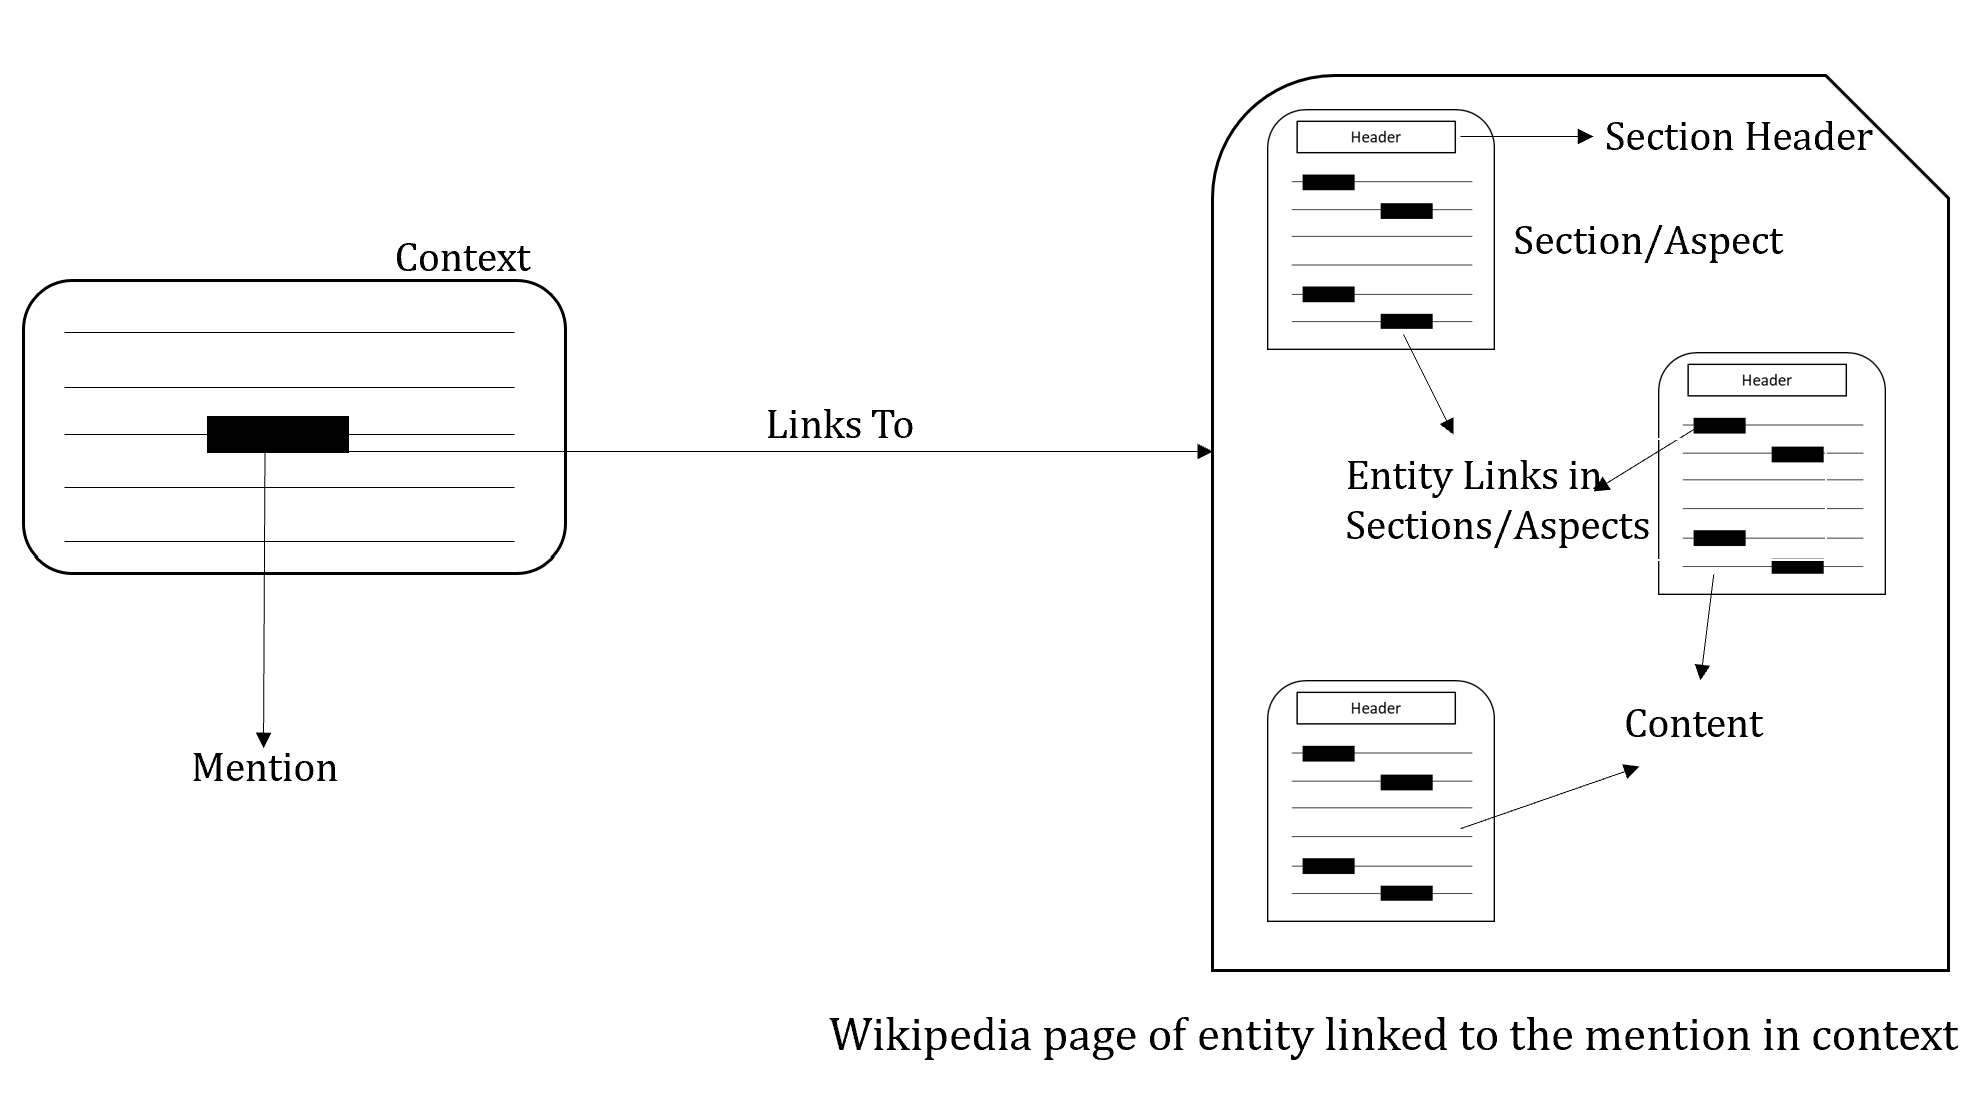
\includegraphics [scale=0.6]{context-and-content.png}
    \caption{Graphical representation of various concepts in aspect linking.}
    \label{fig:context-vs-content}
\end{figure}

Nanni et al. \cite{nanni2018entity} introduce the entity aspect linking task and suggest a combination of text similarity metrics between mention context and aspect content. One of the similarity metrics includes the overlap and similarity of other entities mentioned in context and aspect content. However, their approach would consider all entities equally important for the aspect-linking decision. We believe the approach can be improved by incorporating the entity salience, entity relatedness, and joint aspect linking.  

In context and content, only few entities are salient while most other entities are mentioned in passing, such as in examples, circumstantial references, or clarifications. Approaches for entity salience detection have been developed  recently \cite{dunietz-gillick-2014-new, xiong2018towards, swat} %\ld{cite Dunnietz, cite Xiong, cite SWAT}.
\ld{TODO I made this up, can someone confirm:} In an initial analysis we found that that aspect linking suffers from false-positive aspects which are introduced by spurious entity matches. In this work we explore to which extent salience detection can avoid false positives. We describe entity salience in with an example in Section \ref{subsubsec:Entity salience based features}, when we describe our methods which use salience.
%A detailed introduction to entity salience is given in Section \ref{sec:Background}.

% ruback2018computing : Computing Entity Semantic Similarity by Feature Ranking
% zeng2019measuring : Measuring Entity Relatedness via Entity and Text Joint Embedding : Really well written
% ponza2017two : A two-stage framework for computing entity relatedness in wikipedia : Referenced by a few of the more recent entity relatedness papers I found as "state of the art"
Several entity relatedness measures have been suggested \cite{ristoski2016rdf2vec, ruback2018computing, zeng2019measuring, ponza2017two}. Entity relatedness measures predict the similarity between two entities. We explore if entity relatedness is helpful to link contexts to aspect content whenever they are not mentioning the same entities, but entities that are highly related.
Available entity relatedness tools \cite{piccinno2014wat} are pre-trained from knowledge graphs and do not take the context of the entity mention into account. Nevertheless, we believe that a static entity-relatedness measure will provide robust background knowledge when integrated with indicators from context and content.

The success of modern entity linking tools lies in the integration of contextual entities and their relations in the prediction process \cite{ratinov-etal-2011-local, ferragina2010tagme, hoffart2011robust}. In this paper we incorporate this idea into Entity Aspect Linking: after predicting the aspect-links of entities in the context, we use aspect-to-aspect similarity indicators to improve the aspect linking result of a selected mention. While knowledge graphs naturally provide relations between entities, they are not suitable for describing the relations between entity aspects. Therefore, we explore aspect-to-aspect similarities based on headings, content, and entities. We utilize these similarities to infer the relevance of a particular mention given the context of the linked co-occurring entities.
 
Finally, we reproduce the implementation of Nanni et al.\ and explore several avenues for improvement.


%Nanni et al. \cite{nanni2018entity} have shown that a supervised combination of various text and entity features based on embeddings of the words and entities from various sources (context of mention, content of Wikipedia page of the mention, etc) is able to correctly predict aspects in 70\% of the cases. In this work, we build on their work and use entity salience and relatedness based features in supervised setting with some lexical and semantic features used in \cite{nanni2018entity} and show that this leads to significant improvements in results on the task.

\paragraph{\textbf{Contributions.}} 

%This paper studies the role of entity salience and relatedness on the aspect linking task. We study how these indicators can help and under what conditions they work. We show that using these indicators alone may not be useful but a supervised combination of salience and relatedness based features along with some lexical and semantic features outperforms the current state-of-the-art on the task. We also study the effect of using the frequency and relatedness 
%contextual entities on the task.

Our contributions are as follows.
\begin{itemize}

    \item We study the effect of using entity salience, entity relatedness and co-occurring entities on the task.
    % LD: People think this is obvious that the combination is better than alone, but I think we can make a point here
    %\item We show that although entity salience and entity relatedness can work on their own, a supervised combination of these indicators along with some lexical and semantic features can outperform several baselines and the current state-of-the-art on the task to achieve better results.
    \item We study the benefits of entity salience detection in weighting contextual entities by their importance for the aspect linking decision. 
    \item We incorporate static entity relatedness measures as well as co-occurrence statistics in the entity aspect linking method.
    \item We explore to which extent aspect-to-aspect similarity can be trained and exploited to improve the quality of aspect links. \ld{Jordan: expand/rephrase -- or delete once done}
    \item We analyze the utility of sequence models such as bi-LSTMS with ELMo embeddings in contrast to simple bag-of-words models.
    \item We present a detailed study and analysis of the conditions under which these indicators work versus do not work. 
    \item We offer a reproduction and re-implementation of the entity aspect linking method of Nanni et al. \cite{nanni2018entity}
\end{itemize}

\paragraph{\textbf{Outline.}} The remainder of this paper is organized as follows. Section \ref{sec:Related Work} discusses some related work on the topic. %Section \ref{sec:Background} gives the background information about various components of our approach.
Section \ref{sec:Approach} presents our proposed method in detail. Section \ref{jordan-logistic} introduces the logistic model used in predicting aspect relevance, while Section \ref{jordan-lstm} uses a Bi-LSTM model to predict aspects embedded using ELMo. In Section \ref{jordan-co-entity}, we motivate the use of co-occuring entities in predicting the relevance of aspects in a joint learning model.  Section \ref{sec:Evaluation} presents a quantitative evaluation of our work. Finally, we conclude the paper with Section \ref{sec:Conclusion}.



\section{Related Work}
\label{sec:Related Work}
We provide a brief overview of related work on entity linking, the use of Wikipedia sections for fine-grained annotations, and co-occurrence analysis in passages.

\subsection{Entity Linking}
The task of Entity Linking is to link the mention of an entity in text to a knowledge base entry. Several entity linking systems exist such as TagMe \cite{ferragina2010tagme}, DBPedia Spotlight \cite{mendes2011dbpedia}, Babelfy \cite{babelfy} and WAT \cite{piccinno2014wat}. All these systems examine the context around the entity to disambiguate the entity mention. 
For example, in the sentence \textit{Steve Jobs founded Apple}, the system would predict from the context that the mention \textit{Apple} refers to the company but in the sentence \textit{The apple fell on Newton's head}, the mention \textit{apple} refers to the fruit. 
More recently, systems have been developed to produce embeddings of entities from text and knowledge graphs \cite{huang2015leveraging,ristoski2016rdf2vec,yamada2016joint} and for entity disambiguation and linking \cite{yamada2017learning}. 

In this work, we aim to further enrich an entity link with the correct aspect of the entity mention in the text. We treat the sections from the Wikipedia page of the entity mention as different aspects of the entity and given an entity mention along with the sentence, paragraph and section context, try to link it to the correct section (that is, aspect).

%\textbf{Joint Entity Linking.} In this paper, we consider the use of contextual information from co-occuring entities to aid in linking aspects.

%Durret et al. \cite{durrett2014joint} approach joint entity linking by simultaneously trying to resolve a named entity recognition, entity linking, and co-reference resolution problem. Their joint model uses a structured conditional random field, the context consisting of extracted mentions and text of the document to be linked. In contrast, we take the approach of jointly modeling the relevance of mentions to candidate aspects.

%Nguyen et al. \cite{nguyen2016joint} embed mentions and candidate entities using a Convolutional Neural Network (CNN). Their joint model arises from a sum of local features, which measure the similarity between embedded mentions and candidate entities, and of global features, which are based on the entire collection of mentions and candidate entities in the document.

%Chen Liu et al. \cite{liu2019attention} also use a CNN to embed candidate candidate entities and mentions. They first link the most likely candidates to mentions based on a local measure of relevance. They then use an attention mechanism to determine the most likely candidate for each mention based on these links. While our method is similar, we not only use the highest linked candidate for each mention, but also all candidates and their associated measures of relevance, to infer a global context.

\subsection{Entity Aspect Linking using Sections} 
The following works try to map entities or passages to Wikipedia sections, similar to how we want to map an entity to a Wikipedia section.

Fetahu et al. \cite{fetahu2015automated} enrich Wikipedia sections with news-article references in two steps: First, they suggest news articles to Wikipedia entities (article-entity placement step) and Second, they find the exact section in the entity page where the article must be placed (article-section placement step).

Banerjee et al. \cite{banerjee2015wikikreator} seek to improve Wikipedia stubs by generating content for each section automatically. Their system is based on a text classifier which uses topic distribution vectors to assign content from the web to various sections on a Wikipedia article. This is followed by an abstractive summarization step where section-specific summaries for Wikipedia stubs are generated.

Reinanda et al. \cite{reinanda2016document} present a method for document filtering for long-tail entities, which is based on using aspect-features to identify relevant documents. 

Nanni et al. \cite{nanni2018entity} define each section of the Wikipedia page of the entity as an aspect following \cite{fetahu2015automated,banerjee2015wikikreator,reinanda2016document}.
In their work, they present a learning-to-rank based method which uses both lexical and semantic features derived from various contexts such as the sentence, paragraph and section where the entity is mentioned in text. They use two types of feature-vectors: (a) Word Vector Models, which consider the symbolic representation of each word as a token using TF-IDF and BM25, and rank aspects using the header, content and entity representations and, (b) Distributional Semantic Models, where each word/entity is represented by its embedding for ranking aspects with header and content representations. They show that using lexical and semantic features with different context sizes improves performance over several established baselines. They also showed the usefulness of their method on three downstream applications.  


%They present a learning-to-rank based method which uses both lexical and semantic features derived from various contexts such as the sentence, paragraph and section where the entity is mentioned in text and show that this improves performance over several established baselines. 

In our work, we adopt the same definition of aspects as Nanni  et al. \cite{nanni2018entity} and use their dataset. However, we consider the role of entity salience and relatedness and show that a supervised combination of lexical and semantic features with salience and relatedness features achieves state-of-the-art results.

\subsection{Using Co-occurring Entities}
The following works use entities which co-occur with a given entity in two different tasks and show their effectiveness on the task. 

Dalton et al. \cite{dalton2014entity} present the Entity Context Model (ECM) in their work on Entity Query Feature Expansion. They use the ECM to derive a distribution over words in the context of an entity and co-occurring entities with the entity.

Chatterjee et al. \cite{chatterjee2019why} present the Entity Context Document (ECD) in their work in Entity Support Passage Retrieval.For a given query and entity, they try to find a passage which explains to the user, the relationship between the query and the entity. They show that using frequently co-occurring entities with the target entity (the entity about which the support passage needs to be found) is useful in the task.

Following the idea about using co-occurring entities in \cite{dalton2014entity, chatterjee2019why}, we study the effect of using the frequency and relatedness of co-occurring entities on the entity aspect linking task. In particular, we study whether using the frequency of co-occurrence or the relatedness of the co-occurring entities to a given entity is a better indicator of aspects. 



\section{Background}
\label{sec:Background}
\label{subsubsec:Lexical and Semantic features} 
\label{entity-aspect-representation}

Nanni et al.\cite{nanni2018entity} suggest a range of the lexical and semantic features. Since our method builds on these features, we briefly describe them here.
%al.\cite{nanni2018entity} consider three types of aspect representations and rank aspects based on similarity of mention in context to:(1) Header, (2) Content and, (3) Entity overlap with each section on the Wikipedia page of the entity. They use five methods to derive features from the aspect representations above: (1) TF-IDF, (2) BM25, (3) Word Embeddings, (4) Entity Embeddings, 

Nanni et al. \cite{nanni2018entity} uses a ``bag of words'' vector space model to represent entity aspects. They consider three different ways of comparing the context of the entity mention based on the following entity aspect fields:


\begin{enumerate}

\item \textbf{Header.} Rank aspects based on similarity of the mention in context to the header of each section in the Wikipedia page.

\item \textbf{Content.} Rank aspects based on the similarity between the mention in context and the content of each section of the Wikipedia page of the entity.

\item \textbf{Entity.} Overlap of entities mentioned in the context of the entity mention and the content of a section on the Wikipedia page of the entity.
\end{enumerate}


They use five methods to derive features from these fields: 

\begin{enumerate}
    \item \textbf{TF-IDF} Cosine similarity between the TF-IDF (logarithmic, L2-normalized) vector of contextual mention and aspect field.
    \item \textbf{BM25.} Rank aspect representations using the contextual mention as a query using BM25 ($k_1=2, b=0.75)$.
    \item \textbf{Word embeddings} Cosine similarity between the mention in context and
the aspect using pre-trained GloVe \cite{pennington2014glove} embeddings of dimension 300. 
    \item \textbf{Entity embeddings} Using 500 dimensional RDF2Vec \cite{ristoski2016rdf2vec} embeddings to embed entities in the context of the entity mention and a section from the Wikipedia page of the entity, then compute the document vector using the TF-IDF of an an entity in context of the entity mention and its embedding.
    \item \textbf{Term overlap} Number of shared words after tokenization.
    \item \textbf{Size} a context-independent feature, which is the numbers of words in an entity aspect's text.
\end{enumerate}

Furthermore, they explore different context sizes, sentence, paragraph, and section.


% \textbf{TF-IDF.} Cosine similarity between the TF-IDF (logarithmic, L2-normalized) vector of contextual mention and aspect.

% \textbf{BM25.} Rank aspect representations using the contextual mention as a query using BM25 ($k_1=2, b=0.75)$.

% \textbf{Word Embeddings.} Cosine similarity between the mention in context and
% the aspect using pre-trained GloVe \cite{pennington2014glove} embeddings of dimension 300. 

% \textbf{Entity Embeddings.} Use 500 dimensional RDF2Vec \cite{ristoski2016rdf2vec} embeddings to embed entities in the context of the entity mention and a section from the Wikipedia page of the entity, then compute
% the document vector using the TF-IDF of an an entity in context of the entity mention and its embedding.





%\textbf{entity overlap}. The mention context (the sentence, paragraph, or section that an entity mention occurs in) contains one or more entities. Similarly, the text of each entity aspect also contains entities. We count the number of unique overlapping entities between the mention context an entity aspect.

%\textbf{content overlap.} Similar to the \textbf{entity overlap} feature, we count the number of unique overlapping unigrams between the mention context and the entity aspect's main body of text.

%\textbf{size}. This is simply the number of words contained in an entity aspect's main body of text.

%\textbf{BM25}. The Okapi Best Match 25 (BM25) function is commonly used to rank documents according to relevance to a query. In this paper, the query consists of the mention context (sentence, paragraph, or section), while the documents represent candidate entity aspects. We consider two versions of BM25 dependant on the query field: BM25-header queries the section header of each aspect, while BM25-content queries the main body of text contained in the section that an entity aspect represents.

%\textbf{w-emb. } \ld{third person!} We embed both the mention context and the entity aspect main body of text using Word2Vec. Each embedding consists of the mean embedding of each word contained in the text. The final score is cosine similarity measures between the mention context embedding and the entity aspect embedding. 



\section{Approach}
\label{sec:Approach}
Our goal is to enrich entity links with fine-grained aspects of the entities. In this work, we consider whether a static measure of entity salience and relatedness which has not been trained for this task can help. We refer to the entity that we are trying to aspect link as the target entity.

%To study the role of entity salience, entity relatedness and co-occurring entities, we describe below several ranking strategies based on these and later combine them in a learning-to-rank system. In all our discussions, we refer to the entity that we are trying to aspect link as the target entity.

\subsection{Features}
\label{subsec:Features}

\subsubsection{Entity salience based features}
\label{subsubsec:Entity salience based features}
We use SWAT \cite{swat} to find salience of entities in text. Given a text, SWAT returns the entities in the text along with their salience scores.
\begin{enumerate}
    \item \textbf{Salience of Entity Mention in aspect (Sal-EM).} Score of the aspect is equal to the salience score of the entity mention in the aspect if the entity is salient, and zero otherwise.
    
    \item \textbf{Salient Entities in Context (SEC).} Score an aspect by summing over the salience score of entities $e \in E$, where $E = E_A \cap E_C$, $E_A =$ aspect entities, and $E_C =$ salient entities in sentence, paragraph and section context.
    
    %We use the sentence, paragraph and section context around the entity mention to get the set of salient entities $E_C$ in the context using SWAT. We then find the set of entities $E_A$ in the aspect using WAT\cite{piccinno2014wat}. We then find how many entities in the aspect overlap with the salient entities in the context, $E = E_A \cap E_C$. We then score an aspect by summing over the salience score of common entities in $E$. If no overlap is found, the aspect score is zero.
   %\item \textbf{Salient entities in context.} We use the sentence, paragraph and section context around the entity mention to get the set of salient entities $E_C$ in the context using SWAT. We then find the set of entities $E_A$ in the aspect in two ways: (a) Salient entities using SWAT \cite{swat} \textbf{(SEC-swat)} and (b) All entities using WAT \textbf{(SEC-wat)} \cite{piccinno2014wat}. We then find how many entities in the aspect overlap with the salient entities in the context, $E = E_A \cap E_C$. We then score an aspect by summing over the salience score of common entities in $E$. If no overlap is found, the aspect score is zero. Note, that the context referred to here is the local context of the target entity such as the sentence or paragraph in which the target entity occurs. Later, in Section \ref{subsubsec:Features based on contextual entities}, we use the term contextual entities to refer to other entities which co-occur with the target entity in the entire document collection. The use of the term \textit{contextual} in Section \ref{subsubsec:Features based on contextual entities} should not be confused with the use of the term \textit{context} here.
    
    \item \textbf{All Entities in Context (AEC).} 
    %Same as \ref{subsubsec:Entity salience based features}(2) above, but use both salient and non-salient entities from SWAT for $E_C$.
    To investigate the extent to which salient entities can affect the performance, we also experiment with using both salient and non-salient entities from SWAT for $E_C$ in \ref{subsubsec:Entity salience based features}(2) above. 
\end{enumerate}


\subsubsection{Entity relatedness based features.} 
\label{subsubsec:Entity relatedness based features}
We use WAT \cite{piccinno2014wat} to find relatedness of two entities. Given a list of entities, WAT returns the relatedness between every pair in the list.


\textbf{Co-occurring entities with an entity from context.}
For every entity $e$ in the sentence, paragraph and section context around the target entity $e_T$, we derive a distribution over co-occurring entities $e'$
with $e$ using the frequency of co-occurrence and the relatedness of co-occurring entities to $e$. We may treat this distribution as the conditional probability distribution $P(e' \vert e)$. To find the co-occurring entities, we use the Entity Context Document (ECD) \cite{chatterjee2019why} for $e$. The ECD is created by first retrieving a candidate set of passages using $e$ as the query and then concatenating all passages which mention $e$.
%We find the set of all entities $E$ in the sentence, paragraph and section context around the target entity. For every entity $e \in E$, we derive a distribution over the co-occurring entities $e'$ with $e$. This is done using an initial candidate set of passages retrieved using the entity $e$ as the query (using Lucene defualt BM25) from an index of passages from the TREC Complex Answer Retrieval \cite{dietz2018trec} track dataset. Then we concatenate all passages in the candidate set which mention the entity $e$ as in \cite{dalton2014entity,chatterjee2019why}, to get a composite document of all passages mentioning $e$. We call this composite document as an Entity Context Document (ECD) following Chatterjee et al. \cite{chatterjee2019why}. All entities in this ECD are the co-occurring entities with $e$. We then derive a distribution over co-occurring entities with $e$ in two ways: (a) frequency of co-occurrence, and (b) relatedness of each co-occurring entity $e'$ to the entity $e \in E$. We may treat this distribution as the the conditional probability distribution $P(e' \vert e)$, the conditional probability of seeing the co-occurring entity $e'$ provided that we have already seen the target entity $e$. 
We score an aspect $A$ in following ways.

\begin{enumerate}
    \item \textbf{Simple Frequency Distribution (SF-Dist).} 
   % Score an aspect using
    %\begin{equation}
    %\label{eq:score-aspect-using-simple-freq-dist}
    %    \text{Score(A)} = \sum_{e' \in A}P(e' \vert e)
    %\end{equation}
    %where $e'$ is an entity in the aspect $A$ which also frequently co-occurs with $e$, $e$ is an entity from the context around the target entity $e_T$, and $P( e' \vert e)$ is the frequency distribution over co-occurring
entities.
    
    We score aspects using frequently co-occurring entities with an entity $e$ from the sentence, paragraph and section context around the target entity, which also occur in the aspect content. Formally,:
    \begin{equation}
    \label{eq:score-aspect-using-simple-freq-dist}
        \text{Score(A)} = \sum_{e' \in A}P(e' \vert e)
    \end{equation}
    where $e'$ is an entity in the aspect $A$ which also frequently co-occurs with $e$, $e$ is an entity from the context around the target entity, and $P( e' \vert e)$ is the frequency distribution over co-occurring entities.
    
    \item \textbf{Weighted Frequency Distribution (WF-Dist).} 
    %Same as \ref{subsubsec:Entity relatedness based features}(1) above, but weigh each probability by the relatedness of $e'$ to the target entity $e_T$.
    
    Our intuition is that co-occurring entities which are more related to the target entity should contribute more to the final aspect scores. To investigate how relatedness of co-occurring entities affects the aspect scores, we experiment with scoring an aspect $A$ using a weighted sum of frequencies of entities $e'$ in the aspect, weighted by the relatedness of $e'$ to the target entity $e_T$. Formally,
\begin{equation}
\label{eq:score-aspect-using-weighted-freq-dist}
    \text{Score(A)} = \sum_{e' \in A} \text{Relatedness}(e', e_T) \times P(e' \vert e)
\end{equation}
where $e'$ is an entity in the aspect $A$ which also frequently co-occurs with $e$, $e_T$ is the target entity, $e$ is an entity from the context around the target entity $e_T$, and $\text{Relatedness}(e', e_T)$ is found using WAT \cite{piccinno2014wat}.

\item \textbf{Relatedness Distribution (Rel-Dist).} 
Same as \ref{subsubsec:Entity relatedness based features}(1), but use relatedness of $e'$ to $e$ to find $P( e' \vert e)$.

%Same as \ref{subsubsec:Co-occurring entities based features}(1), but we use the relatedness measure between a co-occurring entity $e'$ and an entity $e$ from the context around the target entity to derive the distribution $P( e' \vert e)$.
\end{enumerate}

\textbf{Co-occurring entities with the target entity.} 
We use two sources of co-occurring entities with the target entity $e_T$: Entity Context Document (\textbf{ECD}) for $e_T$ and the Wikipedia page (\textbf{Wiki}) of $e_T$. We then score an aspect using the co-occurring entities with $e_T$ in two ways.

    
\begin{enumerate}
    \item Use Equation \ref{eq:score-aspect-using-simple-freq-dist} with either frequency distribution \textbf{(SF-Dist-ECD)} or relatedness distribution \textbf{(Rel-Dist-ECD/Rel-Dist-Wiki)} over co-occurring entities to score an aspect.
        
    \item Retrieval Score of Aspect (\textbf{RS-Asp}). We treat the target entity $e_T$ as the query and expand the query using top-20 (according to frequency (\textbf{Freq}) and relatedness (\textbf{Rel})) entities from the ECD/Wikipedia page for $e_T$. We then retrieve aspects from an aspect index for $e_T$ (\textbf{RS-Asp-Freq-ECD/RS-Asp-Rel-ECD/RS-Asp-Rel-Wiki}). We experiment with the combinations of the following retrieval models: BM25 (default Lucene), Language Models with Jelinek-Mercer (LMJM) smoothing $(\lambda = 0.4)$, and Language Models with Dirichlet (LMDS) smoothing, and the following expansion models: RM1 and RM3.
\end{enumerate}
    

\subsubsection{Lexical and Semantic features}
\label{subsubsec:Lexical and Semantic features} 
We re-implemented the lexical and semantic features from Nanni et
al.\cite{nanni2018entity}. To give a brief recap, Nanni et al.\cite{nanni2018entity} consider three types of aspect representations and rank aspects based on similarity of mention in context to:(1) Header, (2) Content and, (3) Entity overlap with each section on the Wikipedia page of the entity. They use four methods to derive features from the aspect representations above: (1) TF-IDF, (2) BM25, (3) Word Embeddings and, (4) Entity Embeddings.

\subsubsection{Jordan's Features} 

\cite{pytorch}
\subsubsection{Neural Network}



\begin{comment}
We give a brief overview of the same again for reference. 

Nanni et al.\cite{nanni2018entity} consider three types of aspect representations for finding its similarity to the entity mention in context. 

\textbf{Header.} Rank aspects based on similarity of the mention in context to the header of each section in the Wikipedia page.

\textbf{Content.} Rank aspects based on the similarity between the mention in context and the content of each section of the Wikipedia page of the entity.

\textbf{Entity.} Overlap of entities mentioned in the context of the entity mention and the content of a section on the Wikipedia page of the entity.

They use the following features to rank aspects using the representations above.

\textbf{TF-IDF.} Cosine similarity between the TF-IDF (logarithmic, L2-normalized) vector of contextual mention and aspect.

\textbf{BM25.} Rank aspect representations using the contextual mention as a query using BM25 ($k_1=2, b=0.75)$.

\textbf{Word Embeddings.} Cosine similarity between the mention in context and
the aspect using pre-trained GloVe \cite{pennington2014glove} embeddings of dimension 300. 

\textbf{Entity Embeddings.} Use 500 dimensional RDF2Vec \cite{ristoski2016rdf2vec} embeddings to embed entities in the context of the entity mention and a section from the Wikipedia page of the entity, then compute
the document vector using the TF-IDF of an an entity in context of the entity mention and its embedding.
\end{comment}

\newcommand{\todo}[1]{\textcolor{red}{TODO: #1}\PackageWarning{TODO:}{#1!}}

\section{Evaluation}
\label{sec:Evaluation}
In this section, a quantitative evaluation of our system is presented on the entity-aspect dataset from Nanni et al.\cite{nanni2018entity}. We begin by presenting some research questions pertaining to three broad components of our system: Entity Salience, Entity Relatedness and Co-occurring entities, which our experiments aim to address(Section \ref{subsec:Research Questions}). We then describe our experimental settings (Section \ref{subsec:Evaluation Paradigm}), followed by the baselines (Section \ref{subsec:Baselines}). We end this section with a discussion of our experiments and results (Section \ref{subsec:Results}).

\subsection{Research Questions}
\label{subsec:Research Questions}

\begin{itemize}
\item[\textbf{RQ1}] Does entity salience affect the task? If yes, then to what extent?
\item[\textbf{RQ2}] Does entity relatedness affect the task? If yes, then to what extent? 
\item[\textbf{RQ3}] Is the frequency or relatedness of co-occurring entities a better indicator of a good aspect?
\item[\textbf{RQ4}] Can we use co-occurring entities to infer the correct entity aspect?
\item[\textbf{RQ5}] Does filtering out non-relevant co-occurring entities improve results when inferring the correct entity aspect?
\end{itemize}

\subsection{Evaluation Paradigm}
\label{subsec:Evaluation Paradigm}

\textbf{Datasets.} Due to the lack of other datasets in this area, we use the Entity Aspect Linking dataset from Nanni et al.\cite{nanni2018entity}. It consists of 201 entity mentions from Wikipedia along with their sentence, paragraph and section context and a list of candidate aspects for the mention. We use this dataset for training a L2R algorithm using 5-fold cross validation. 

We use the TREC Complex Answer Retrieval (CAR) track \cite{dietz2018trec}\footnote{\url{http://trec-car.cs.unh.edu}} dataset as a source of passages when building the Entity Context Document in Section \ref{subsubsec:Entity relatedness based features}. It consists of an entity linked corpus consisting of paragraphs from the entire English Wikipedia. 

Since neural networks require large training data to perform well and the dataset from Nanni et al. \cite{nanni2018entity} contains only 201 entity mention, we construct our own training data using the \textit{AllButBenchmark} from TREC CAR. \textit{AllButBenchmark} consists of nearly whole of Wikipedia (all pages and all sections on those pages along with the images embedded on the page), except for pages which were included in the official evaluation topics for years during which the track was active at TREC.

Our new training data consists of 88,000 training examples extracted from the page data in \textit{AllButBenchmark}. It was constructed by retaining entity links within Wikipedia pages that link to top-level sections in other Wikipedia pages, after filtering out for irrelevant sections (such as ``References'', ``See Also'', etc.). We did not filter out self-referential links (a link to another section in the same page). The dataset is modelled after Nanni et al.\cite{nanni2018entity}. Each example contains the sentence context, paragraph context, entity mention and candidate aspects. The candidate aspects are the top level sections of the Wikipedia page of the entity linked to the mention. Each candidate aspect contains information about its section header, text, and entities that are contained within it.


%For each example in which an entity in a paragraph links to a section in a page, the candidate aspects for the example are the top level sections where the ground truth is the section that was linked to. Each example contains the sentence context, paragraph context and entity mention that contains the link to a different section. Each candidate represents a section, and contains information about its section header, text, and entities that are contained within it.
    
%These consist of entity links within Wikipedia pages that link to top-level sections in other Wikipedia pages, after filtering out for irrelevant sections (such as ``References'', ``See Also'', etc.). We did not filter out self-referential links (a link to another section in the same page). 
    


\textbf{Ground Truth.} The dataset from Nanni et al. \cite{nanni2018entity} contains a ground truth file which maps a mention to the correct aspect. %The TREC Complex Answer Retrieval track \cite{dietz2018trec} dataset contains both passage and entity ground truth data. 
The ground truth for our new training data was constructed in a similar way: the true aspect of an entity mention is the top-level section on the Wikipedia page of the entity linked to the mention and in which the mention appears.

\textbf{Evaluation Metrics.} We use Precision at 1 (P@1) and Mean Reciprocal Rank (MRR) as our evaluation metrics.

\textbf{Entity Linking.} Both data sets contain the entities from Wikipedia mentioned in the context and aspect content. In addition, we use WAT \cite{piccinno2014wat} to annotate the context and aspect content to get more entities. 

\textbf{Entity Salience Detection.} We use SWAT \cite{swat}  to find the salience of an entity in text. Given some text, SWAT outputs the entities along with their salience scores in the text. For example, using the online demo \footnote{https://swat.d4science.org/}, given the two passages in Figure \ref{fig:Salience}, SWAT correctly predicts \textit{Boris Johnson} as salient in Passage 2 (Score = 0.6), and non-salient in Passage 1 (Score = 0.15). 

\textbf{Entity Relatedness Detection.} We use the Entity Relatedness system from WAT \cite{piccinno2014wat} to find relatedness between pairs of entities. Given a list of entities, WAT provides the relatedness measure between every pair of entities in the list. For example, given the entity list consisting of \textit{Boris Johnson}, \textit{Theresa May} and \textit{Donald Trump}, WAT predicts the relatedness between every pair of entities as follows:
\begin{quote}
    (\text{Boris Johnson}, \text{Donald Trump}) = 0.37, \\
    (\text{Theresa May},\text{Donald Trump})    = 0.38, \\
    (\text{Boris Johnson}, \text{Theresa May})  = 0.67
\end{quote}

\textbf{Machine Learning.}
We apply our methods to produce an aspect ranking for every entity mention. We then treat each ranking as a feature and perform 5-fold cross validation with a listwise learning-to-rank (L2R) method (Coordinate Ascent) optimized for Precision at 1 (P@1). We use RankLib\footnote{Dang, V. "The Lemur Project-Wiki-RankLib." Lemur Project,[Online]. Available: \url{http://sourceforge. net/p/lemur/wiki/RankLib}.} for this purpose. 

\ld{Jordan's stuff...}
\textbf{Neural Methods.}
We evaluate the Logistic Network, BiLSTM network, and Global Context Separately, as well as together with respect to joint optimization. We train each model with respect to binary cross entropy, using the Adam optimizer from the PyTorch library. We use samples from the 88k dataset, and then evaluate with respect to the samples in Nanni et al.'s dataset. We report P@1 and MAP statistics for each method. The \textbf{just-logistic, just-bi,} and \textbf{just-global} methods are with respect to evaluation using only the logistic network, BiLSTM network, and global context network respectively. The \textbf{joint-network} method consists of all three networks, the parameters of which are trained simultaneously.
\ld{End of Jordan's stuff...}

\subsection{Baselines}
\label{subsec:Baselines}

\textbf{Baseline 1: Nanni et al.} We re-implement all features from Nanni et al. \cite{nanni2018entity} and use a supervised combination of sentence, paragraph and section context features as our baselines. \\
\textbf{Baseline 2: Size.} We consider the length of each section (in number of tokens) and link the entity-mention to the longest. \\
%\textbf{Baseline 3: Content Overlap.} Overlap between the tokens in the sentence, paragraph and section context of the mention. \\
%\textbf{Baseline 4: Entity Overlap.} Overlap between the entities in the sentence, paragraph and section context of the mention. \\

\subsection{Results}
\label{subsec:Results}
The most interesting results are presented in Table \ref{tab:Results}. Due to space constraints other results were moved to the online appendix for this paper. Below, we discuss each of the research questions presented in Section \ref{subsec:Research Questions}.
%Below, we discuss results from our experiments with respect to the three broad components of our system: entity salience, entity relatedness and co-occurring entities, and answer the research questions presented in Section \ref{subsec:Research Questions}.


\begin{figure}
    \centering
    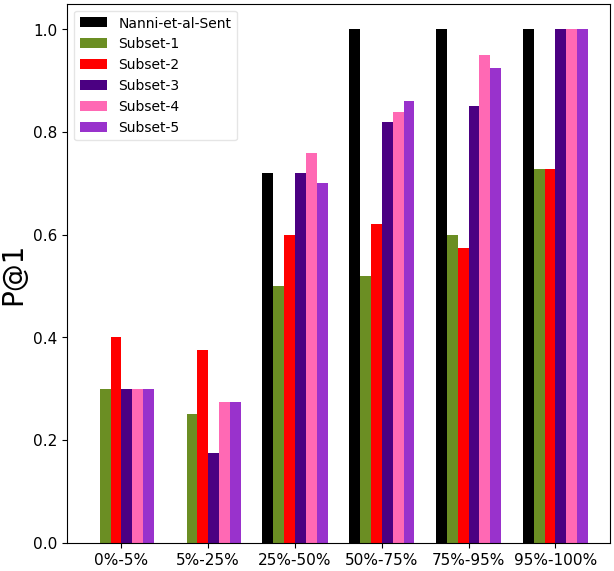
\includegraphics [scale=0.5]{plot-cropped.png}
    \caption{Difficulty-test for P@1, comparing Nanni et al.(Sentence) to various L2R systems.}
    \label{fig:difficulty-plot}
\end{figure}

\begin{table}[]
\caption{Performance of individual entity rankings (in terms of MAP) on different contexts obtained using frequency and relatedness and combined with L2R.}
\label{tab:Results-Entity-Rankings-Freq-And-Rel}
\begin{tabular}{@{}llll@{}}
 \toprule
            & Sentence & Paragraph & Section \\ \midrule
Frequency   & 0.04     & 0.06      & 0.13    \\
Relatedness & 0.03     & 0.03      & 0.04    \\ \midrule
L2R         & 0.01     & 0.02      & 0.03   \\
 \bottomrule
\end{tabular}
\end{table}



\begin{table}[t]
\caption{Performance of individual entity rankings (in terms of MAP) on different contexts obtained using entity salience and combined with L2R.}
\label{tab:Results-Entity-Rankings-Sal}
\begin{tabular}{@{}llll@{}}
\toprule
                                & Sentence & Paragraph & Section \\ \midrule
Context-Salient-Content-Salient & 0.002    & 0.001     & 0.003   \\
Context-Salient-Content-All     & 0.009    & 0.005     & 0.008   \\
Context-All-Content-Salient     & 0.006    & 0.008     & 0.003   \\
Context-All-Content-All         & 0.02     & 0.02      & 0.01    \\ \midrule
L2R                             & 0.006    & 0.009     & 0.005   \\ \bottomrule
\end{tabular}
\end{table}

\begin{table}[t]
\caption{Helps-Hurts analysis for frequency versus salience.}
\label{tab:Helps-Hurts-Analysis}
\begin{tabular}{|l|c|c|c|c|c|c|}
\hline
                                & \multicolumn{6}{c|}{Relatedness}                                                              \\ \hline
                                & \multicolumn{2}{c|}{Sentence} & \multicolumn{2}{c|}{Paragraph} & \multicolumn{2}{c|}{Section} \\ \hline
                                & Helps         & Hurts         & Helps          & Hurts         & Helps         & Hurts        \\ \hline
\multicolumn{1}{|c|}{Frequency} & 679           & 15            & 1018           & 9             & 1160          & 3            \\ \hline
\end{tabular}
\end{table}

\begin{table*}[t]
\caption{Results from Nanni et al.\cite{nanni2018entity} and from our implementation of their methods.}
\label{tab:Reproducible-results}
\begin{tabular}{|c|c|c|c|c|c|c|}
\hline
                          &               &               &                &               &               &               \\ \hline
                          & \multicolumn{2}{c|}{Sentence} & \multicolumn{2}{c|}{Paragraph} & \multicolumn{2}{c|}{Section}  \\ \hline
                          & P@1           & MRR           & P@1            & MRR           & P@1           & MRR           \\ \hline
Original (from the paper) & 0.70$\pm$0.03 & 0.81$\pm$0.02 & 0.65$\pm$0.03  & 0.78$\pm$0.03 & 0.57$\pm$0.03 & 0.73$\pm$0.03 \\ \hline
Re-implemented            & 0.67$\pm$0.03 & 0.79$\pm$0.02 & 0.64$\pm$0.03  & 0.78$\pm$0.03 & 0.53$\pm$0.03 & 0.71$\pm$0.03 \\ \hline
\end{tabular}
\end{table*}

\begin{table}[t]
    \caption{Performance with standard error of individual entity salience and relatedness features and combined with L2R, including subsets/ablations.}
    \label{tab:Results-shubham}
    %\scalebox{0.9}{
    \begin{tabular}{@{}lllll@{}}
        \toprule
        Method & P@1 & MRR \\ 
        
        \midrule
        
        Nanni et al. (Sentence) &
        0.67$\pm$0.03 & 0.79$\pm$0.02 \\
        
         Nanni et al. (Paragraph) &
        0.64$\pm$0.03  & 0.78$\pm$0.03 \\
        
         Nanni et al. (Section) &
       0.53$\pm$0.03 & 0.71$\pm$0.03 \\
     
      Size &
      0.39$\pm$0.03&
      0.60$\pm$0.03
      \\
      
      \midrule
      
     
    Sal-EM   &   
      0.19$\pm$0.03 &
      0.46$\pm$0.03
      \\
      
      
      
      SEC (Sentence)  &    
      0.23$\pm$0.03 &
      0.53$\pm$0.03
      \\
      
      
      AEC (Sentence)   &    
      0.51$\pm$0.03 &
      0.70$\pm$0.03
      \\
       \midrule
      
     
      SF-Dist (Sentence)   &    
      0.54$\pm$0.03 &
      0.72$\pm$0.03
      \\
      
     
      WF-Dist (Sentence)  &    
      0.49$\pm$0.03 &
      0.67$\pm$0.03
      \\
      
      
      Rel-Dist (Sentence)  &    
      0.43$\pm$0.03 &
     0.62$\pm$0.03
      \\
       \midrule
      
    
      SF-Dist-ECD   &    
      0.35$\pm$0.03 &
      0.59$\pm$0.03
      \\
      
      
      Rel-Dist-ECD  &    
      0.36$\pm$0.03 &
      0.60$\pm$0.03
      \\
      
     
      RS-Asp-Freq-ECD (LMJM + RM1)  &     
      0.35$\pm$0.03 &
      0.59$\pm$0.03
      \\
      
       
      RS-Asp-Rel-ECD (LMJM + RM1) &     
      0.40$\pm$0.03 &
      0.60$\pm$0.03
      \\
       \midrule
      
      
      Rel-Dist-Wiki  &    
      0.37$\pm$0.03 &
      0.60$\pm$0.03
      \\
      
      
       
      RS-Asp-Rel-Wiki (BM25 + RM3)  &     
      0.39$\pm$0.03 &
      0.61$\pm$0.03
      \\
      \midrule
      
       Subset-1 (Only Relatedness) &
      0.48$\pm$0.03 &
      0.68$\pm$0.03
      \\
      
      
      Subset-2 (Only Salience) &
      0.59$\pm$0.03 &
      0.72$\pm$0.03
      \\
      
       Subset-3 (Rel. + Lex. + Sem.) &
      0.66$\pm$0.03 &
      0.78$\pm$0.03
      \\
      
       Subset-4 (Sal + Lex. + Sem.) &
      
      0.72$\pm$0.03 &
      0.82$\pm$0.03
      \\
      
      
      Subset-5 (Sal. + Rel. + Lex. + Sem.) &
      0.70$\pm$0.03 &
      0.81$\pm$0.03
      \\
     
      
      

     
      
       \bottomrule
    \end{tabular}
    %}
\end{table}

\todo{Jordan: Add your results to another table here.}

\subsubsection{Reproduction of Nanni et al.}
\label{subsubsec:Reproduction of Nanni et al}
\todo{Jordan: Add some text here.}


\subsubsection{Entity Salience}
\label{subsubsec:Entity Salience}
%\textbf{RQ1: Entity Salience.}

\paragraph{\textbf{Observations.}}
We observe from Table \ref{tab:Results-shubham} that a supervised combination of all salience features (Subset-2) outperforms 2 of the 4 baselines, whereas a combination of all salience features with the lexical and semantic features (Subset-4) outperforms all baselines. However, considering all entities (salient and non-salient) in the context (AEC Sentence) performs better than considering only the salient entities (SEC Sentence). We also find that in Subset-2, learning-to-rank always places maximum weight on the AEC methods.

\paragraph{\textbf{Discussions.}}
These observations show the effectiveness of using salience. However, they also indicate that considering non-salient entities together with the salient ones help improve performance. To investigate this further, we manually confirmed that SWAT correctly identifies salient entities in text. However, SWAT returns more empty results when asked for only salient entities than when asked for all (salient or otherwise) entities. For example, using the sentence context of an entity mention, it returns an empty result for 100 of the 201 entity mentions when asked for only the salient entities and 13 of 201 entity mentions when asked for all  entities. This shows the limitations in SWAT and why the results obtained using \textit{SEC (Sentence)} is lower than \textit{AEC (Sentence)}.  Our intuition is that the other entities, although non-salient, have some inherent semantic meaning and hence considering them together with the salient entities helps the task. This is the case for the paragraph and section contexts too but we do not show the results here due to space constraints. 

Moreover, in Section \ref{subsec:Entity Salience for Aspect Linking}, we match the salient entities in the context to (1) salient entities in the aspect (SEC), and (2) all entities in the aspect (AEC). Matching through SEC gives us very few entities for the aspect, whereas matching through AEC gives us more entities. However, the entities obtained through SEC are salient whereas a lot of entities obtained through AEC are not important (non-salient). Ideally, one would train a L2R model to learn how much weight to put on each alternative. Here we present an additional experiment where we produce an entity ranking for each aspect using four alternatives: (1) Match salient entities in context to salient entities in aspect, (2) Match salient entities in context to all entities in aspect, (3) Match all entities in context to salient entities in aspect and (4) Match all entities in context to all entities in aspect. We evaluate these entity rankings using a ``ground truth" of aspects where we define any entity mentioned in the aspect as relevant for the aspect. The results are shown in Table \ref{tab:Results-Entity-Rankings-Sal}. 

Consider the two passages in Figure \ref{fig:Salience} from two news articles about the entity \textit{Boris Johnson} which address his role as the \textit{Prime Minister of the UK} and his response to the recent COVID-19 pandemic.
\begin{figure}[t]
    \centering
   \begin{quote}
\textbf{Passage 1.} The British government came under heightened pressure to disclose details about a secretive scientific advisory group after a report on Friday that a top political aide to Prime Minister Boris Johnson had taken part in the group’s meetings on the coronavirus pandemic. \\
\textbf{Passage 2.} British Prime Minister Boris Johnson is resisting growing calls to reopen the UK from its lockdown because he is still so “frightened” from his own near-fatal brush with the bug, according to a report .
\end{quote}
    \caption{Salient versus Non-Salient Passage. Passage 2 is salient for entity \textit{Boris Johnson} whereas Passage 1 is not.}
    \label{fig:Salience}
\end{figure}
We notice that Passage 2 \footnote{https://nypost.com/2020/04/21/boris-johnson-too-frightened-to-ease-uk-coronavirus-lockdown/} in Figure \ref{fig:Salience} discusses how the entity \textit{Boris Johnson} in his role as the Prime Minister of the UK is affecting the pandemic situation, whereas Passage 1 \footnote{https://www.nytimes.com/2020/04/25/world/europe/uk-dominic-cummings-sage-coronavirus.html} just mentions the entity on the side. The entity is central to the discussion in Passage 2 whereas in Passage 1, it is not. We say that \textit{Boris Johnson} is \textit{salient} in Passage 2. Hence, by \textit{salient}, we mean that the entity is \textit{central} to the text in which it is mentioned. 

Consider the following sentence from a new article about \textit{Boris Johnson}.

\begin{quote}
    \textit{Boris Johnson, perhaps the world's most famous coronavirus patient, was back at work Monday — after spending the worst of Britain's epidemic sidelined,
first in self-isolation, then struggling to breathe in the hospital, and later in recovery in the countryside \footnote{https://www.washingtonpost.com/world/europe/boris-johnson-returns-to-work-after-missing-worst-of-coronavirus-epidemic/2020/04/27/95b590ea-8630-11ea-81a3-9690c9881111_story.html}}.
\end{quote}

In a sentence such as the one above, we would not only prefer to link the mention \textit{Boris Johnson} to the aspect \textit{Prime Minister of the UK}, but also to one in which the entity is salient. 

We observe in Table \ref{tab:Results-Entity-Rankings-Sal} that matching all entities in context to all entities in aspect works the best. This is expected because as discussed above, we lose a lot of entities when asking SWAT for only salient entities. Moreover, matching salient context entities to all aspect entities works better than matching with only salient aspect entities. For example, matching salient context entities to all aspect entities using sentence context has $\text{MAP}=0.009$, whereas matching with salient aspect entities has $\text{MAP}=0.002$. Although these numbers are not very encouraging, they depict that matching salient context entities to all aspect entities is better. This also shows why AEC outperforms SEC in Table \ref{tab:Results-shubham}.

%we observe that the L2R combination of these entity rankings for each context type performs very poorly.
One issue with matching entities in such an exact way is that very often, there are no matches. In such cases, a lot of aspects receive a score of zero in our methods (SEC and AEC in Section \ref{subsec:Entity Salience for Aspect Linking}). This also shows why the \textit{AEC (Sentence)} outperforms  \textit{SEC (Sentence)} in Table \ref{tab:Results-shubham}. There are more matching entities when matching all aspect entities (as in AEC) than when matching only salient aspect entities (as in SEC), with salient context entities, as evident by the MAP results for methods \textit{Context-Salient-Content-Salient} and \textit{Context-Salient-Content-All} in Table \ref{tab:Results-Entity-Rankings-Sal}. To illustrate this issue, we present an example from the dataset of Nanni et al.\cite{nanni2018entity} that we used in our work in Figure \ref{fig:Salience-Example}. We observe that the entity \textit{Kyoto Protocol} is salient in the context (shown by bold italic) but not in the content (shown by only bold). Hence, SEC would score this aspect zero since there are no matching salient entities, but AEC would not.


To investigate the extent to which salience helps, we divide the entity mentions  into different levels of difficulty according to the performance (P@1) of the \textit{Nanni et al. (Sentence)} method, with the 5\% most difficult queries fo
r this method to the left and the 5\% easiest ones to the right, and compare the performance with the \textit{Subset-4}. The results are shown in Figure \ref{fig:difficulty-plot}. We observe that whenever it is difficult to perform the task using \textit{Nanni et al. (Sentence)}, entity salience supports our L2R system (Subset-2 and Subset-4).


\paragraph{\textbf{Conclusions.}}
With respect to RQ1, we can say that entity salience does indeed affect the task positively. We are able to outperform all the baselines with the help of salience and we see that salience helps to boost performance when the queries get difficult by learning information which is complimentary to the lexical and semantic features. However, exactly matching entities between context and aspect content leads to finding no matches for most aspects and hence most aspects receive a score of zero. Added to this are the limitations of SWAT in finding salient entities. Hence, entity salience is helpful but hindered by we need to know how to use it to help our task.

%We are able to outperform all the baselines with the help of salience and we see that salience helps to boost performance when the queries get difficult. However, SWAT is still limited in its salience detection and this hinders the performance of a system using it. 

%\textbf{RQ2: Entity Relatedness.}
\subsubsection{Entity Relatedness}
\label{subsubsec:Entity Relatedness}

\paragraph{\textbf{Observations.}}
We observe from Table \ref{tab:Results-shubham} that a supervised combination of all relatedness features (Subset-1) does not perform very well on its own, doing better than only one baseline (Size). However, a combination of relatedness features with the lexical and semantic features (Subset-3) does significantly better than 3 of the 4 baselines. Moreover, a combination of salience and relatedness features with the lexical and semantic features outperforms all baselines. 

\paragraph{\textbf{Discussions.}}
These observations indicate that entity relatedness does indeed affect the task positively. However, salience is more informative than relatedness as is evident from the superior performance of Subset-2 over Subset-1 and Subset-4 over Subset-3. On further investigation, we found that WAT finds many false positives and false negatives. For example, given the entity list consisting of  \textit{World War I}, \textit{Vietnam War} and \textit{France}, it predicts that \textit{World War I} is related to \textit{Vietnam War} (false positive) but  unrelated to \textit{France} (false negative). This is because WAT does not take
the query or the context of the entity into account but makes predictions based on certain graph-based features such as number of inlinks and outlinks to and
from a particular entity node in a knowledge graph. 

To investigate the extent to which relatedness helps, we present results from the difficulty test explained in Section \ref{subsubsec:Entity Salience} in Figure \ref{fig:difficulty-plot}. We observe that whenever it is difficult to perform the task using \textit{Nanni et al. (Sentence)}, entity relatedness supports our L2R system (Subset-3 and Subset-5).


\paragraph{\textbf{Conclusions.}}
With respect to RQ2, we may say that relatedness does indeed affect the task positively. Although relatedness of entities by itself may not perform very well, a supervised combination with lexical and semantic features improves performance over several baselines. Moreover, a L2R system containing relatedness based features help to boost performance when queries get difficult. However, the limitations of WAT hinder the performance of a system using it.

%considering relatedness features in combination with some lexical and semantic features can help the task. However, WAT is limited in its entity relatedness system where it finds many false positives and false negatives.

%\textbf{RQ3: Frequency vs Relatedness.}
\subsubsection{Frequency vs Relatedness}
\label{Frequency vs Relatedness}

\paragraph{\textbf{Observations.}}
From Table \ref{tab:Results-shubham}, we observe that ranking aspects using \textit{SF-Dist (Sentence)} outperforms \textit{WF-Dist (Sentence)}, which in turn outperforms \textit{Rel-Dist (Sentence)}). Moreover, \textit{RS-Asp-Freq-ECD} outperforms \textit{RS-Asp-Rel-ECD}. We also find that when L2R is trained on all relatedness features (Subset-1), it places more weight on the features using frequency distribution those using relatedness. 

\paragraph{\textbf{Discussions.}}
These observations indicate that using the frequency of co-occurring entities is more informative than the relatedness. To investigate this further, as in Section \ref{subsubsec:Entity Salience}, we produce entity rankings for every aspect using (1) frequency (SF-Dist in Section \ref{subsec:Entity Relatedness for Aspect Linking}(1)) and (2) relatedness (Rel-Dist in Section \ref{subsec:Entity Relatedness for Aspect Linking}(3)) of entities and evaluate these rankings by defining all entities in an aspect as relevant for the aspect. The results are shown in Table \ref{tab:Results-Entity-Rankings-Freq-And-Rel}.

From Table \ref{tab:Results-Entity-Rankings-Freq-And-Rel}, we observe that the entity rankings obtained using frequency distribution are indeed better (in terms of Mean Average Precision (MAP)) than those obtained using relatedness. For example, entity ranking obtained using section context and frequency distribution has $\text{MAP}=0.13$ whereas that obtained using relatedness has $\text{MAP}=0.04$. We also perform an additional experiment where we analyse the number of aspects that were helped (in terms of MAP) by using frequency distribution of co-occurring entities as compared to using the relatedness distribution. The results are shown in Table \ref{tab:Helps-Hurts-Analysis}. We observe, for example, that using frequency with section context helps 1160 aspects while hurting just 3 as compared to using relatedness. This shows why the entity ranking obtained using frequency and section context performs better than that obtained using relatedness in Table \ref{tab:Results-Entity-Rankings-Freq-And-Rel},and consequently, why the \textit{SF-Dist} methods perform better than the \textit{Rel-Dist} method in Table \ref{tab:Results-shubham}.

\paragraph{\textbf{Conclusions.}}
With respect to RQ3, we may say that using frequency of co-occurring entities is better than using relatedness because most frequently co-occurring entities are also related but most related entities do not frequently co-occur. Moreover, with respect to RQ2, although relatedness can help when the queries get difficult, as compared to frequency, it hurts the performance of a method using it.
 

%%
% The first command in your LaTeX source must be the \documentclass command.
\documentclass[sigconf,authordraft]{acmart}
\usepackage{booktabs}
\usepackage{verbatim}
\usepackage{graphicx}

 %activate todo's
\newcommand{\todo}[1]{\textcolor{red}{TODO: #1}\PackageWarning{TODO:}{#1!}}
% deactivate todos
%\newcommand{\todo}[1]{ \PackageWarning{TODO:}{#1!}}

%
% defining the \BibTeX command - from Oren Patashnik's original BibTeX documentation.
\def\BibTeX{{\rm B\kern-.05em{\sc i\kern-.025em b}\kern-.08emT\kern-.1667em\lower.7ex\hbox{E}\kern-.125emX}}
    
% Rights management information. 
% This information is sent to you when you complete the rights form.
% These commands have SAMPLE values in them; it is your responsibility as an author to replace the commands and values with those provided to you when you complete the rights form.
%
% These commands are for a PROCEEDINGS abstract or paper.
\copyrightyear{2018}
\acmYear{2018}
\setcopyright{acmlicensed}
\acmConference[Woodstock '18]{Woodstock '18: ACM Symposium on Neural Gaze Detection}{June 03--05, 2018}{Woodstock, NY}
\acmBooktitle{Woodstock '18: ACM Symposium on Neural Gaze Detection, June 03--05, 2018, Woodstock, NY}
\acmPrice{15.00}
\acmDOI{10.1145/1122445.1122456}
\acmISBN{978-1-4503-9999-9/18/06}


\begin{document}

% P@1: 0.606, MAP: 0.761

\bibliographystyle{ACM-Reference-Format}
\bibliography{references}
\end{document}


  

\section{Conclusion}
\label{sec:Conclusion}
This work addresses the task of entity aspect linking and studies the effectiveness of using entity salience and relatedness on the task using two off-the-shelf tools not trained for this task. We show that although these tools are not perfect and do not pose a solution on their own, a supervised combination of salience and relatedness features with lexical and semantic features can outperform several established baselines. In particular, we show that such a supervised combination learns complementary information which aids the performance of the supervised system. Moreover, we find that using the frequency of co-occurring entities is better than using their relatedness since frequently co-occurring entities are mostly related, but related entities might not co-occur frequently. 

Despite this success, we believe that there is potential for further improvement, if salience detection and entity relatedness would be customized for the entity aspect linking task. One issue is that relatedness is both unaware of the context and the aspect content. Extending entity relatedness measures to consider relatedness-in-context (similarly to the prominence score) is likely to offer further improvements. Analogously, salience detection is currently trained for a linguistic purpose, that is unaware of the downstream task. We speculate that developing a new salience-like component that can identify which entities in the context are sufficiently central to be incorporated in the matching decision. Both a context-ware entity relatedness and a task-aware salience detector---once available---would also be useful for other downstream tasks.

Overall, we believe that our contribution to entity aspect-linking contributes to new knowledge-based information access systems. For once, it allows to construct knowledge graphs on the sub-entity level. While the edges are not typed, the fine-grained aspects model the roles that entities play in multi-way relations. Furthermore entity-aspect linking allows better information access for journalists, researchers, as well as any users who is seeking to understand fine-grained connections between entities through their aspects for open-domain information needs.

\bibliographystyle{ACM-Reference-Format}
\bibliography{references}

\end{document}
